\documentclass{article}
\usepackage{fancyhdr} % Required for custom headers
\usepackage{lastpage} % Required to determine the last page for the footer
\usepackage{extramarks} % Required for headers and footers
\usepackage{graphicx} % Required to insert images
%\usepackage{lipsum} % Used for inserting dummy 'Lorem ipsum' text into the template
\usepackage{amsmath}
%\usepackage{amsfont}
%\usepackage{amssymb}

\usepackage{multicol}
% Margins
\topmargin=-0.5in
\evensidemargin=0in
\oddsidemargin=-0.5in
\textwidth=7.5in
\textheight=9.0in
\headsep=0.25in 


\pagestyle{fancy}

\rhead{M. Adam} % Top right header
\lhead{Shrimp Pad Tai}
\chead{ }
%\title{}

\begin{document}
%
%PRELIMINARIES:
%
%
%Begin by preheating the oven to 350 $^o$F
%
%\bigskip
%
%\bigskip

\begin{multicols}{2}
Ingredients:
\begin{itemize}
\item 3/4 pound wild prawns (shelled and deveined)
\item 5 tbsp sesame oil
\item 2 garlic cloves, chopped
\item 1/2 small white onion or 1 shallot, chopped
\item 1 fresh serrano chile, processed through garlic press
\item 1/8 tsp paprika
\item 2 eggs
\item Salt and pepper to taste
\item 16 oz. rice noodles
\item 4 cups boiling water
\end{itemize}

For the sauce:
\begin{itemize}
\item Juice of 2 fresh limes
\item 2.5 tbsp sugar
\item 3 tbsp fish sauce
\end{itemize}

To garnish:
\begin{itemize}
\item 1/2 cup fresh cilantro, chopped
\item 1 cup mung bean sprouts
\item 4 lime wedges
\item 1/4 cup chopped peanuts (optional)
\end{itemize}

\columnbreak

Directions:
\begin{enumerate}
\item In a large pot boil water. Place the rice noodles in a large bowl (heat resistant) and pour the boiling water over the noodles, let the noodle cook for approximately 5-10 minutes. After 10 minutes stir the noodle in the water to prevent from sticking. Set aside without draining the water.

\item Over med high heat, add in sesame oil to the pan, sauté the shallots and garlic for about 1 minute. Prep the serrano chili by removing the seeds and process through garlic press.

\item Add chile to the pan and cook for another minute, add prawns with small amount of salt and pepper and sauté them for 1-2 minutes or until they turn pink and opaque.

\item To make the sauce, in a bowl, mix together fresh lime juice, sugar, and fish sauce, set aside.

\item Flip the prawns over sprinkle paprika and toss them, cook for another 1-2 minutes. When the tails of the prawns are pink and the prawns are bouncy they are done. Place prawns into a bowl and set aside.

\item In a small bowl crack eggs and break the yolk. In the same pan add the rest of the sesame oil and lightly scramble the eggs. Remove the pan from the heat and turn down the heat to low.

\item Strain the noodles.

\item Place the pan back on top of the heat, add prawns, noodles, and drizzle the sauce over. Gently toss the noodles until the sauce is all soaked into the noodles.

\item Garnish with mung bean sprouts, cilantro, lime wedges, and peanuts.
\end{enumerate}
\end{multicols}



\begin{center}
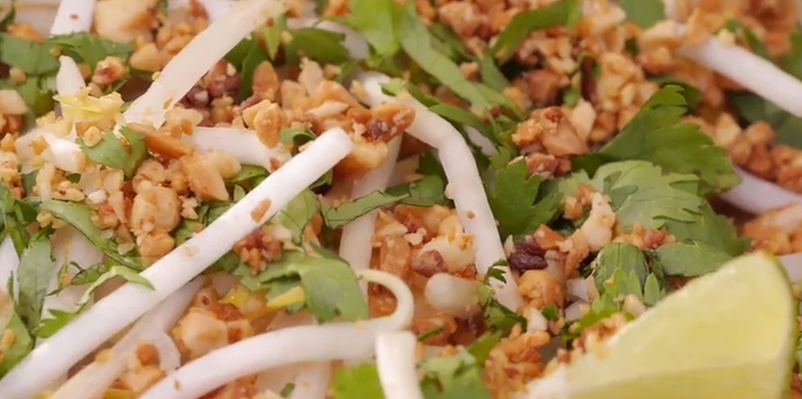
\includegraphics[scale=0.4]{ShrimpPadTai.png}
\end{center}


\end{document} 











